\lecture{14}{7 Feb.\ 11:00}{\(L^1\) Space}
\section{\(L^1\) Space}
We now introduce another space called \emph{\(L^p\) spaces}, which are function spaces defined using a natural generalization of the \hyperref[eg:p-norm]{\(p\)-norm} for finite-dimensional vector spaces. We sometimes call it Lebesgue spaces also. Before we start, we need to define a \emph{norm}.

\begin{definition}[Norm]\label{def:norm}
	Let \(V\) be a vector space over filed \(\mathbb{R} \) or \(\mathbb{C} \). A \emph{norm} is a \hyperref[def:seminorm]{seminorm}
	\begin{definition}[Seminorm]\label{def:seminorm}
		A \emph{seminorm} on \(V\) is
		\[
			\left\lVert \cdot\right\rVert \colon V\to [0, \infty )
		\]
		such that
		\begin{itemize}
			\item \(\left\lVert c v\right\rVert =\left\vert c \right\vert \left\lVert v\right\rVert \) for every \(v\in V\) and every scalar \(c\).
			\item \(\left\lVert  v+w\right\rVert \leq \left\lVert v\right\rVert +\left\lVert w\right\rVert \) for every \(v, w\in V\).
		\end{itemize}
	\end{definition}
	with an additional condition
	\begin{itemize}
		\item \(\left\lVert v\right\rVert = 0 \iff v = 0\).
	\end{itemize}
\end{definition}

\begin{lemma}
	A \hyperref[def:norm]{normed} vector space is a metric space with metric \(\rho (v, w) = \left\lVert v - w\right\rVert\).
\end{lemma}
\begin{proof}
	\todo{DIY}
\end{proof}

\begin{eg}[\(p\)-norm]\label{eg:p-norm}
	\(V = \mathbb{R} ^d\) with
	\[
		\left\lVert x\right\rVert _p = \begin{dcases}
			\left(\sum_{i=1}^{d} \left\vert x_{i} \right\vert^p \right)^{1/p}, & \text{ if }  p\in[0, \infty ); \\
			\max_{1\leq i\leq d} \left\vert x_{i} \right\vert ,                & \text{ if } p = \infty
		\end{dcases}
	\]
	is a \hyperref[def:norm]{normed} vector space. The unit ball
	\[
		\{x\in\mathbb{R} ^d \mid \left\lVert x\right\rVert _p\leq 1\}
	\]
	for different \(p\) has the following figures.
	\begin{figure}[H]
		\centering
		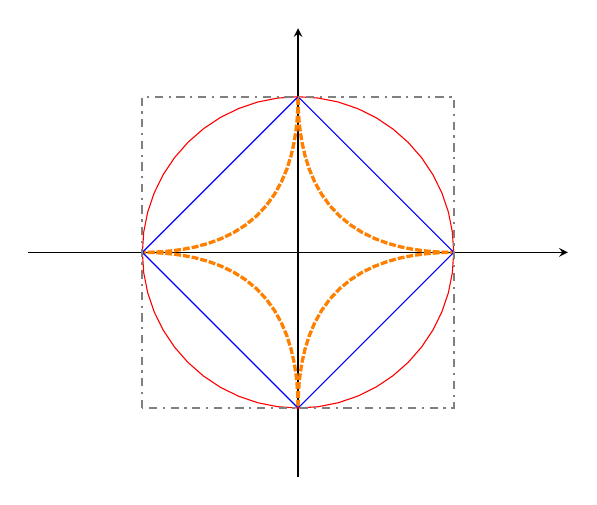
\begin{tikzpicture}
			\begin{axis}[axis lines=middle,xtick=\empty,ytick=\empty,axis equal,enlargelimits,xmax=1.2,ymax=1.2,xmin=-1.2,ymin=-1.2]
				%p=0.5
				\begin{scope}[very thick,dotted,orange,domain=0:pi,samples=50]
					\addplot[] ({(cos(deg(x)))^(4},{ (sin(deg(x))^(4});
					\addplot[] ({(cos(deg(x)))^(4},{ -(sin(deg(x))^(4});
					\addplot[] ({-(cos(deg(x)))^(4},{ (sin(deg(x))^(4});
					\addplot[] ({-(cos(deg(x)))^(4},{-(sin(deg(x))^(4});
				\end{scope}
				%p=1
				\addplot[blue,domain=0:pi] ({(cos(deg(x)))^2},{(sin(deg(x))^2});
				\addplot[blue,domain=0:pi] ({(cos(deg(x)))^2},{-(sin(deg(x))^2});
				\addplot[blue,domain=0:pi] ({-(cos(deg(x)))^2},{(sin(deg(x))^2});
				\addplot[blue,domain=0:pi] ({-(cos(deg(x)))^2},{-(sin(deg(x))^2});
				%p=2
				\addplot[red,domain=-pi:0] ({(cos(deg(x)))},{(sin(deg(x))});
				\addplot[red,domain=0:pi] ({(cos(deg(x)))},{(sin(deg(x))});
				%p=inf
				\draw[thick,dashdotted,gray] (axis cs:-1,-1) rectangle (axis cs:1,1);
			\end{axis}
		\end{tikzpicture}
	\end{figure}
	\begin{remark}
		All \(p\)-norms induce the same topology. i.e., if \(U\) is open in \(p\)-norm, it is open in \(p ^\prime\)-norm
		as well.
	\end{remark}
\end{eg}

\begin{note}
	Recall that we say \(f\) is \hyperref[def:integrable]{integrable} means
	\[
		\int \left\vert f \right\vert <\infty,
	\]
	and if \(f = g\) \hyperref[def:mu-almost-everywhere]{a.e.}, then
	\[
		\int f = \int g
	\]
\end{note}

\begin{definition}[\(L^1\) Space]\label{def:L1-space}
	Given \((X, \mathcal{A} , \mu )\),
	\[
		f\in L^1(X, \mathcal{A} , \mu )\left( = L^1(X, \mu ) = L^1(X) = L^1(\mu )\right)
	\]
	means that \(f\) is an \hyperref[def:integrable]{integrable} function on \(X\).
\end{definition}

\begin{lemma}
	\(L^1(X, \mathcal{A} , \mu )\) is a vector space with \hyperref[def:seminorm]{seminorm}
	\[
		\left\lVert f\right\rVert _1 = \int \left\vert f \right\vert .
	\]
\end{lemma}
\begin{proof}
	\todo{Check this is indeed a \hyperref[def:seminorm]{seminorm}.}
\end{proof}

\begin{definition}[\(L^1\) Space with equivalence class]\label{def:L1-space-equivalence-class}
	Define \(f\sim g\) if \(f = g\) \hyperref[def:mu-almost-everywhere]{a.e.}, then
	\[
		\quotient{L^1(X, \mathcal{A} , \mu )}{\sim} = L^1(X, \mathcal{A} , \mu ),
	\]
	i.e., we simply denote the collection of equivalence classes by itself.\footnote{By some abusing of notation of \(L^1\).}
\end{definition}
\begin{remark}
	We have
	\begin{itemize}
		\item With \autoref{def:L1-space-equivalence-class}, \(L^1(X, \mathcal{A} , \mu )\) is a \hyperref[def:norm]{normed} vector space.
		\item \label{def:L-1-metric} We say that the \emph{\(L^1\)-metric} \(\rho (f, g)\) is simply
		      \[
			      \rho (f, g) = \int \left\vert f - g \right\vert.
		      \]
	\end{itemize}
\end{remark}

\subsubsection{Dense Subsets of \(L^1\)}
\begin{note}
	Recall the definition of a \href{https://en.wikipedia.org/wiki/Dense_set}{\emph{dense set}}.
\end{note}

\begin{definition}[Step function]\label{def:step-function}
	A \emph{step function} on \(\mathbb{R} \) is
	\[
		\psi = \sum_{i=1}^{N} c_{i}\mathbbm{1}_{I_{i}},
	\]
	where \(I_{i}\) is an \underline{interval}.
\end{definition}

\begin{notation}
	We denote the collection of continuous functions \underline{with compact} \hyperref[def:support]{support} by \(C_c(\mathbb{R} )\).
\end{notation}

\begin{theorem}
	We have the following.
	\begin{enumerate}[(a)]
		\item \(\{\text{\hyperref[def:integrable]{integrable} \hyperref[def:simple-function]{simple} functions} \}\) is dense
		      in \(L^1(X, \mathcal{A} , \mu )\) (with respect to \hyperref[def:L-1-metric]{\(L^1\)-metric}).
		\item \((X, \mathcal{A} , \mu ) = (\mathbb{R} , \mathcal{A} _\mu , \mu )\),
		      where \(\mu\) is a \hyperref[def:Lebesgue-Stieltjes-measure]{Lebesgue-Stieltjes-measure}. Then
		      the set of \hyperref[def:integrable]{integrable} \hyperref[def:simple-function]{simple} functions
		      is dense in \(L^1(\mathbb{R} , \mathcal{A} _\mu , \mu )\).
		\item \(C_c(\mathbb{R} )\) is dense in \(L^1(\mathbb{R} , \hyperref[def:Lebesgue-measure]{\mathcal{L} , m})\).
	\end{enumerate}
\end{theorem}
\begin{proof}
	We prove this one by one.
	\begin{enumerate}[(a)]
		\item Since there exists \hyperref[def:simple-function]{simple functions} \(0\leq \left\vert \phi _1 \right\vert \leq \left\vert \phi _2 \right\vert\leq \dots \leq \left\vert f \right\vert  \),
		      where \(\phi _{n}\to f\) \hyperref[def:pointwise-convergence]{pointwise}. Then by \autoref{thm:DCT}, we have
		      \[
			      \lim_{n \to \infty} \int \underbrace{\left\vert f_{n} - f\right\vert }_{\leq \left\vert \phi _{n} \right\vert + \left\vert f  \right\vert\leq 2\left\vert f \right\vert } = 0
		      \]
		      where \(2\left\vert f \right\vert \) is in \(L^1\).
		\item Let \(\mathbbm{1}_{E} \) \underline{approximate} by \(\sum_{i=1}^{\infty} c_{i}\mathbbm{1}_{I_{i}} \). From \autoref{thm:regularity} for
		      \hyperref[def:Lebesgue-Stieltjes-measure]{Lebesgue-Stieltjes-measure},
		      \[
			      \forall \epsilon ^\prime >0\ \exists I = \bigcup_{i=1}^{N} I_{i}\text{ such that } \mu (E\triangle I)\leq \epsilon ^\prime .
		      \]
		\item To approximate \(\mathbbm{1}_{(a, b)} \), we simply consider function \(g\in C_c(\mathbb{R} )\) such that
		      \[
			      \int \left\vert \mathbbm{1}_{(a, b)} - g \right\vert \leq \frac{\epsilon}{2} + \frac{\epsilon}{2} = \epsilon .
		      \]
	\end{enumerate}
\end{proof}